\section{Methods}\label{sec:project}

As already outlined in \autoref{sec:motivation}, this project will study the extent to which hate, discrimination, and racism influence German rap. For this purpose, we would like to use different methods of text analysis, which will be explained in more detail below. The described approach will also be supplemented by a visual representation in \autoref{fig:pipeline}.

\begin{figure}[!htb]
  \centering
  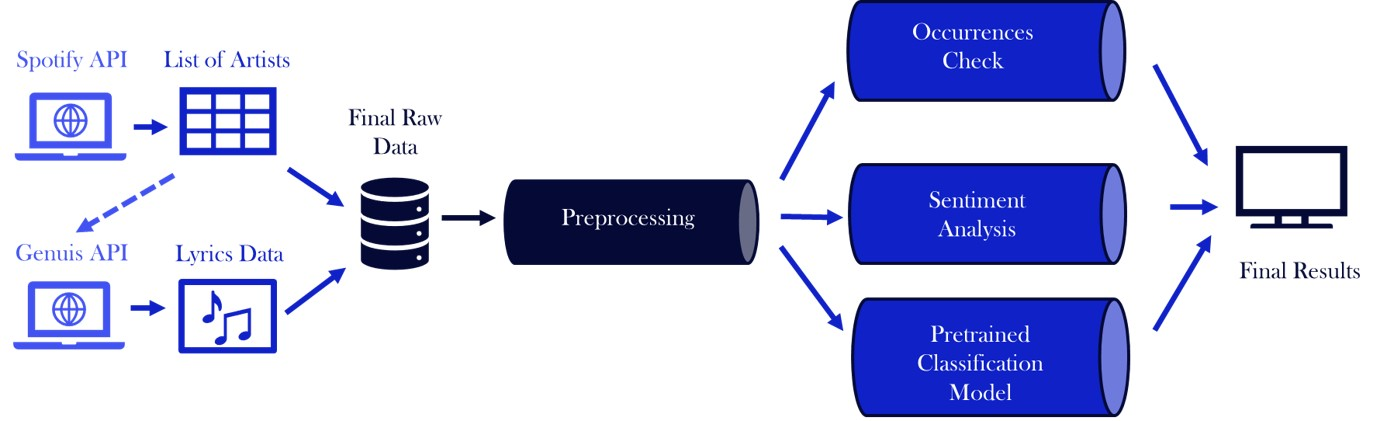
\includegraphics[width=\textwidth]{figures/pipeline.jpg}
  \caption[]{Text Analytics Pipeline}
  \label{fig:pipeline}
  \end{figure}

As a basis for our investigations, a data set on certain artists of the German Rap will be used, which is not finally defined yet. This will be done in the nearest future using information from the web in manual and partially automated work. Corresponding information about artists can be extracted, for example, from \cite{last.fm,tonspion_2021}. The names of those artists are used in a further step to download the lyrics of all songs of those artists via the song lyrics platform Genius \cite{genius}. Genius is an online database for any kind of artistic texts and offers an API interface that provides license-free lyrics of many song lyrics. Since Genius does not fully provide all the data of every international artist, it might be necessary to accept limitations for some artists.

The song lyrics, enriched with information about the artists themselves, finally form the basis of our textual analyses: Since we would like to use pretrained models for the analysis of the lyrics in a further step and many of these models only support English-language texts, it might be necessary to translate the German song lyrics first. For this, we intend to use the Python framework DL Translate \cite{lu_2022}, since it is the only package that can freely translate unlimited texts. The translated lyrics, will be stored together with the original lyrics in ElasticSearch. It must be taken into account that by using such a translation tool, possible linguistic-relevant contexts will be incorrectly transferred into the English language. However, since there is considerable interpretative space in the context of song lyrics, this limitation should not be of too much importance. In fact, it is important to keep in mind for the entire project that the song lyrics studied allow for different interpretations, which can only be determined by machine analysis to a limited extent.

As indicated in the paragraph before, we would like to store the translated song lyrics together with the original data in ElasticSearch. The possibilities that ElasticSearch offers in the area of tokenization, classification of words including counting of word frequencies, etc. shall then be used as a basis for a first analysis of the song lyrics.

In addition to the described methods offered by ElasticSearch, we would like to use predefined machine learning models to enrich the data of the song lyrics. In this context, the frameworks used should be considered as a black box, and the corresponding methods remain untouched. We will consider the following frameworks:

The project Deep Learning Models for Multilingual Hate Speech Detection \cite{deepMLhatespeech} includes multiple models that can be trained or fine-tuned for recognizing hate speech in various languages, especially German. Performing hate detection using different machine learning algorithms in parallel would enable a more thorough analysis of the texts like: highlighting songs that get a high hate rate from most models, identifying common patterns between such songs and classifying them into subclasses according to the target of the hate speech (foreigners, women, disabled people etc.).

The German Sentiment classification with BERT \cite{guhr2020training} is a sentiment classification model trained on around 1.8 million German-language text samples coming from various sources (social media, movie, app and hotel reviews). It could be a starting point for identifying potential hateful song lyrics. Given the three sentiment classes used by this model (negative, neutral and positive), we could filter out texts classified as positive and also separate negative from neutral lyrics for the upcoming pipeline stages.

NLTK.Vader \cite{vader} is an NLP algorithm trained for performing sentiment analysis. It is best suited for short texts like posts on social media, containing some slang and abbreviations. Hence, our dataset on German song lyrics would make a good fit for this model (providing we first use a translation model like mBart \cite{mBart}).

HateSonar \cite{davidson2017automated} is a BERT based model built with Python for hate speech detection. It only works with English data, therefore the German song lyrics would first need to be translated. As with models trained on German texts, it would be beneficial to the analysis to extract information regarding hate speech from multiple models.

If there is time left, we would like to develop independent machine learning models on our own using the methods discussed in the lecture. However, this requires classification of the existing lyrics data, which would likely need to be done manually. Furthermore, the amount of data available could prove challenging with this approach. If it is not feasible to identify a very large number of song lyrics using the listed approach above, it could be difficult to develop meaningful machine learning models.

Finally, the results of the different analysis methods will be interpreted and visualized. Thereby, the findings of the analyses shall be explicitly highlighted using the lyrics data by visual markers. Additionally, results of the different metrics will be displayed. 